\documentclass{llncs}
\usepackage{fullpage}

%load needed packages
\usepackage{graphicx}
\usepackage{array}
\usepackage{booktabs}
\usepackage[utf8]{inputenc}


\begin{document}

\title{Microarray Data Analysis: Summary}

\author{Lukáš Hofman}
\institute{\email{lukas.hofman@uma.es} \\
Aprendizaje Computacional. Universidad de Málaga.}

\maketitle 

\vspace{1cm} % Space down the title

\textit{This report summarizes the key aspects of microarray data
analysis techniques as described in the Basic microarray analysis: Grouping and feature
reduction. Soumya Raychaudhuri; Patrick D. Sutphin;
Jeffrey T. Chang; Russ B. Altman. Trends in Biotechnology.
2001; 19(5):189-193. The summary focuses on how we can summarize and pick out
important details out of large data sets, specifically using supervised and unsupervised learning.}

% This is a comment

\section{Introduction}

\textbf{Microarray analysis is an essential tool for understanding mRNA expression
across various conditions. The technique generates large datasets that require
advanced computational techniques to extract meaningful biological insights.
The two main approaches for analyzing microarray data are supervised and unsupervised 
methods.}


\section{Methods for Grouping Microarray Data}

\subsection{Unsupervised Methods}

Unsupervised methods like clustering group data points based solely on the
patterns present in the data itself. One commonly used method is K-means
clustering, which was applied to a set of lymphoma profiles in the paper to
uncover two distinct subtypes of lymphoma.
Unsupervised methods, unsupervised learning are used for exploratory tasks.

Unsupervised methods:

\begin{itemize}
  \item K-means
  \item Principal component analysis (PCA)  
\end{itemize}

\subsection{Supervised Methods}

Supervised methods, such as classification, require pre-existing labels for
the grouping process. In the paper, Linear Discriminant Analysis (LDA) was
used to classify lymphoma samples based on a set of known examples.
Supervised learning is excellent for answering direct questions (classification)

Supervised methods:

\begin{enumerate}
  \item Linear discriminant analysis (LDA)
  \item Logistic regression
\end{enumerate}


\newcolumntype{C}{>{\centering\arraybackslash} m{5cm} }
\begin{table}
    \label{tab:example1}
 	\caption{Clustering Methods and Results}
	\centering
	\begin{tabular}{C|CCC}
 		\toprule
 		Method & Description & Results \\
 		\midrule
 		K-means Clustering  & Grouped lymphoma profiles using 148 germinal-center genes & 2 clusters: germinal-cell type, activated subtype \\
   		Principal Component Analysis (PCA) & Reduced the dataset to two principal components & Clear separation between subtypes \\
		Linear Discriminant Analysis (LDA) & Classified unknown cases based on known labels & Predicted 2 subtypes with high accuracy \\
 		\bottomrule
 	\end{tabular}
\end{table}

\section{Feature Reduction}

Feature reduction is crucial for simplifying complex datasets. By selecting only
the most informative features, computational complexity is reduced while main-
taining the ability to draw accurate conclusions. In the paper, principal compo-
nent analysis (PCA) was used to reduce the dimensionality of the dataset.

\begin{figure}
	\centering
	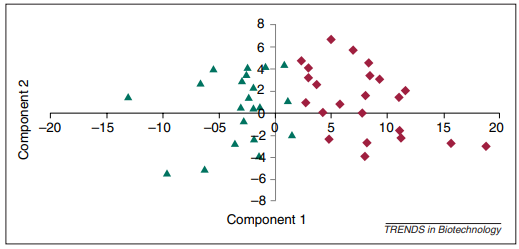
\includegraphics[width=0.75\textwidth]{images/148_to_2_dimensions_lymphoma.png}
	\caption{Visualization of 148 dimensional lymphoma data to 2 dimensions using the PCA to reduce the dimensions.}
	\label{fig:example1}
\end{figure}

\section{Conclusion}

Microarray data analysis is an evolving field that relies on various computational
techniques to make sense of large datasets. The discussed paper demonstrates
the use of clustering and classification techniques as well as feature reduction
to distinguish between cancer subtypes.
These methods are critical for advancing our understanding of biological systems.

\end{document}
